\documentclass[a4paper, 11pt]{article}
\usepackage{geometry}
\geometry{letterpaper, margin=1in}
\usepackage{amsmath}
\usepackage{amssymb}  
\usepackage{amsthm}
\usepackage{ulem} 
\usepackage{graphicx}
\graphicspath{ {images/} }
\usepackage{tikz} 
\begin{document}
%Header-Make sure you update this information!!!!
\noindent
\large\textbf{Thermal Physics - PH441} \hfill \textbf{John Waczak} \\
\normalsize Day 11 \hfill  Date: \today \\

\subsection*{Paramagnetism}
	What is a paramagnetic system? It's a system of a bunch of spins: $\uparrow \downarrow \uparrow \uparrow ...$ where M is the total magnetic moment and m is the magnetic moment of one spin particle. The real tricky part is how do we write the partition function for N spins? One way is to do it as follows: 
		\begin{align*}
			Z &= \sum_\mu e^{-\beta E_\mu} \\ 
		\end{align*}
	If there are 5 spins then we have $2^5$ microstates. Then we can write our partition function can be written as: 
		\begin{align*}
			Z &= \sum_{s_1} \sum_{s_2} \sum_{s_3}\sum_{s_4}\sum_{s_5} e^{-\beta m B(s_1+s_2+s_3+s_4+s_5)} \quad \text{where } s = \pm 1 \\ 
				&= \sum_{s_1}e^{-\beta m B s_1} \sum_{s_2} e^{-\beta m B s_2}\sum_{s_3}e^{-\beta m B s_3}\sum_{s_4}e^{-\beta m B s_4}\sum_{s_5}e^{-\beta m B s_5} \\ 
				&= \Big(\sum_{s}e^{-\beta m B s}\Big)^5 \Rightarrow \Big(\sum_{s}e^{-\beta m B s}\Big)^N = (e^{-\beta m B}+e^{\beta m B})^N \text{ for N spin systems} 
		\end{align*} 
	
\subsection*{Black body radiation} 
	A \textit{black body} is an object that absorbs all radiation incident upon it. Black bodies are interesting because they have universal properties and there are a lot of ways to make something that is black. The simplest example is just a hole! 
		\begin{figure}[!hbt]
			\centering 
			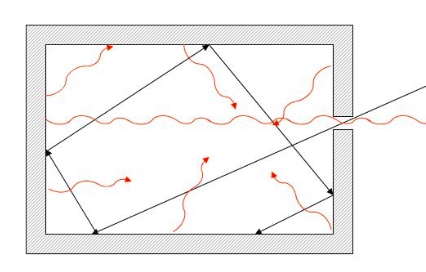
\includegraphics[width=0.35\columnwidth]{blackBody}
			\caption{A "black" hole in a box... kek}
		\end{figure}
	
	\noindent Now we want to figure out what are the eigenstates of energy in a black-box? First we want to know the normal-modes. Then we can figure out the rest! Kuttel's book goes into much more detail and he uses non periodic boundary conditions. David like's periodic boundary systems so we will use those. \\
	
	\noindent Recall the dispersion relation $\omega = c|\vec{k}|$. If we have periodic boundary conditions then we need an integer number of wavelengths in a box (not half integer!). Thus $\frac{2\pi}{k_x} =\lambda \Rightarrow \lambda n_x = L$. Thus $k_x = \frac{2\pi n_x}{L}$. Also note that $n_x =in (-\infty, \infty)$. This means we are allowing traveling waves not just standing waves. Now we can enumerate all of the modes: 
		\begin{align*}
			\omega_{n_xn_yn_z} = \frac{c2\pi}{L}\sqrt{n_x^2+n_y^2+n_z^2}
		\end{align*}
	\noindent Now let's find the partition function. \textbf{Note:} we are summing over all of the micro states not the normal modes... Also because we can have polarizations in two directions we are also missing a hidden factor of 2 in our counting which we will include later. Our state is defined by the number of photons in each of these modes.
		\begin{align*}
			Z &= \sum\limits_{n_{00-1}=0}^\infty\sum\limits_{n_{001}=0}^\infty...\sum\limits_{n_{\pm\infty \pm\infty \pm\infty}=0}^\infty e^{-\beta (\hbar\omega_{001}n_{001}+\hbar\omega_{00-1}n_{00-1}...\hbar\omega_{\pm\infty\pm\infty\pm\infty}n_{\pm\infty\pm\infty\pm\infty})} \\ 
			&= \Big(\sum\limits_{n_{001}}e^{-\beta\hbar\omega_{001}n_{001}}\Big)\Big(\sum\limits_{n_{00-1}}e^{-\beta\hbar\omega_{00-1}n_{00-1}}\Big)...\Big(\sum\limits_{n_{\pm\infty\pm\infty\pm\infty}}e^{-\beta\hbar\omega_{\pm\infty\pm\infty\pm\infty}n_{\pm\infty\pm\infty\pm\infty}}\Big)
		\end{align*}
	\noindent Now each of these is just a simple harmonic oscillator which we have solved for (geometric series) already. 
		\begin{align*}
			Z &= \prod\limits_{n_x=-\infty}^\infty\prod\limits_{n_y=-\infty}^\infty\prod\limits_{n_z=-\infty}^\infty \sum\limits_{n_{n_xn_yn_z}}^{\infty} e^{-\beta\hbar\omega_{n_xn_yn_z}n_{n_xn_yn_z}}
		\end{align*}
	Now we'll square everything to cover that two polarizations business 
		\begin{align*}
			&= \Big(\prod\limits_{n_x=-\infty}^\infty\prod\limits_{n_y=-\infty}^\infty\prod\limits_{n_z=-\infty}^\infty \sum\limits_{n_{n_xn_yn_z}}^{\infty} e^{-\beta\hbar\omega_{n_xn_yn_z}n_{n_xn_yn_z}}\Big)^2 \\ 
			&= \Big(\prod\limits_{n_x=-\infty}^\infty\prod\limits_{n_y=-\infty}^\infty\prod\limits_{n_z=-\infty}^\infty \frac{1}{1-e^{-\beta\hbar\omega_{n_xn_yn_z}}}\Big)^2
		\end{align*}		
	\noindent Now we have everything to figure out the free energy
		\begin{align*}
			F &= -kT\ln Z = 2kT\Big[\sum\limits_{n_x=-\infty}^\infty\sum\limits_{n_y=-\infty}^\infty\sum\limits_{n_z=-\infty}^\infty\ln(1-e^{-\beta\hbar\omega_{n_xn_yn_z}})\Big]\\
			&= 2kT\Big[\sum\limits_{n_x=-\infty}^\infty\sum\limits_{n_y=-\infty}^\infty\sum\limits_{n_z=-\infty}^\infty\ln\Big(1-e^{-\beta\hbar\frac{c2\pi\sqrt{n_x^2+n_y^2+n_z^2}}{L}}\Big)\Big]\\
		\end{align*}
	\noindent Now we can argue that for large L we can turn this sum into a triple integral. 
			
			
			
			
			
			
			
			
			
			
			
			
			
			
			
			
			
			
			
			
			
			
			
			
			
			
			
\end{document}